\part{Getting started}
\section{Signposts}
\textit{River Architect} serves for the GIS-based planning of habitat enhancing stream restoration features regarding their lifespans, design characteristics, optimum placement in the terrain, and ecological benefit. A main graphical user interface (GUI) provides five modules for generating lifespan and design maps, action (optimum lifespan) maps, terrain modification (terraforming) assessment of digital elevation models (DEM), habitat evaluation, and project cost-benefit analyses.\\

\textbf{Lifespan maps} indicate the expected longevity of restoration features as a function of terrain change, morphological characteristics, and 2D hydrodynamic modeling results. \textbf{Design maps} are a side product of lifespan mapping and indicate required feature dimensions for stability, such as the minimum required size of angular boulders to avoid their mobilization during floods \citep[see Part~\ref{part:lf} and ][]{schwindt19a}.\\
\textbf{Action maps} result from the comparison of lifespan and design maps of multiple restoration features and assign features with the highest longevity to each pixel of a raster. Thus, the \textit{Action Planner} module assess optimum features as a function of highest lifespans among comparable feature groups such as terraforming or vegetation planting species(see Part~\ref{part:ap}).\\
The \textbf{Terrain Modification} module prepares DEMs of particular reaches for or after the virtual application of stream restoration features. Moreover, this module can compare "exiting" (pre-project) and "with implementation" (post-feature application) Rasters to determine required earth movement (terraforming) works (see Part~\ref{part:mt}).\\
The \textbf{Habitat Evaluation} module applies a user-defined set of discharges for the spatial evaluation of the habitat suitability index (HSI). The hydraulic habitat suitability results from 2D hydrodynamic numerical model outputs of flow depth and velocity. In addition, the option "cover" can be used to assess cobble, boulder, vegetation and streamwood habitats (see Part~\ref{part:he}).\\
The \textbf{Project Maker} module evaluates the costs for gained area in usable habitat for target fish species and lifestages. A unit cost workbook provides relevant costs and the gain in usable habitat area results from the \textit{Habitat Evaluation} module. The usage of the \textit{Project Maker} module is explained in Part ~\ref{part:pm}.\\
A set of \textbf{Tools} provides console Python scripts to generate required input files and to support terraforming drawing efforts.\\

Fig.~\ref{fig:flowchart} shows a flowchart for the application of \textit{River Architect}'s modules and external input data for designing habitat enhancement projects. The modules and tool-scripts can also be individually applied for other purposes than suggested in the flowchart.\\

\begin{figure}[!hbt]
	\begin{center}
	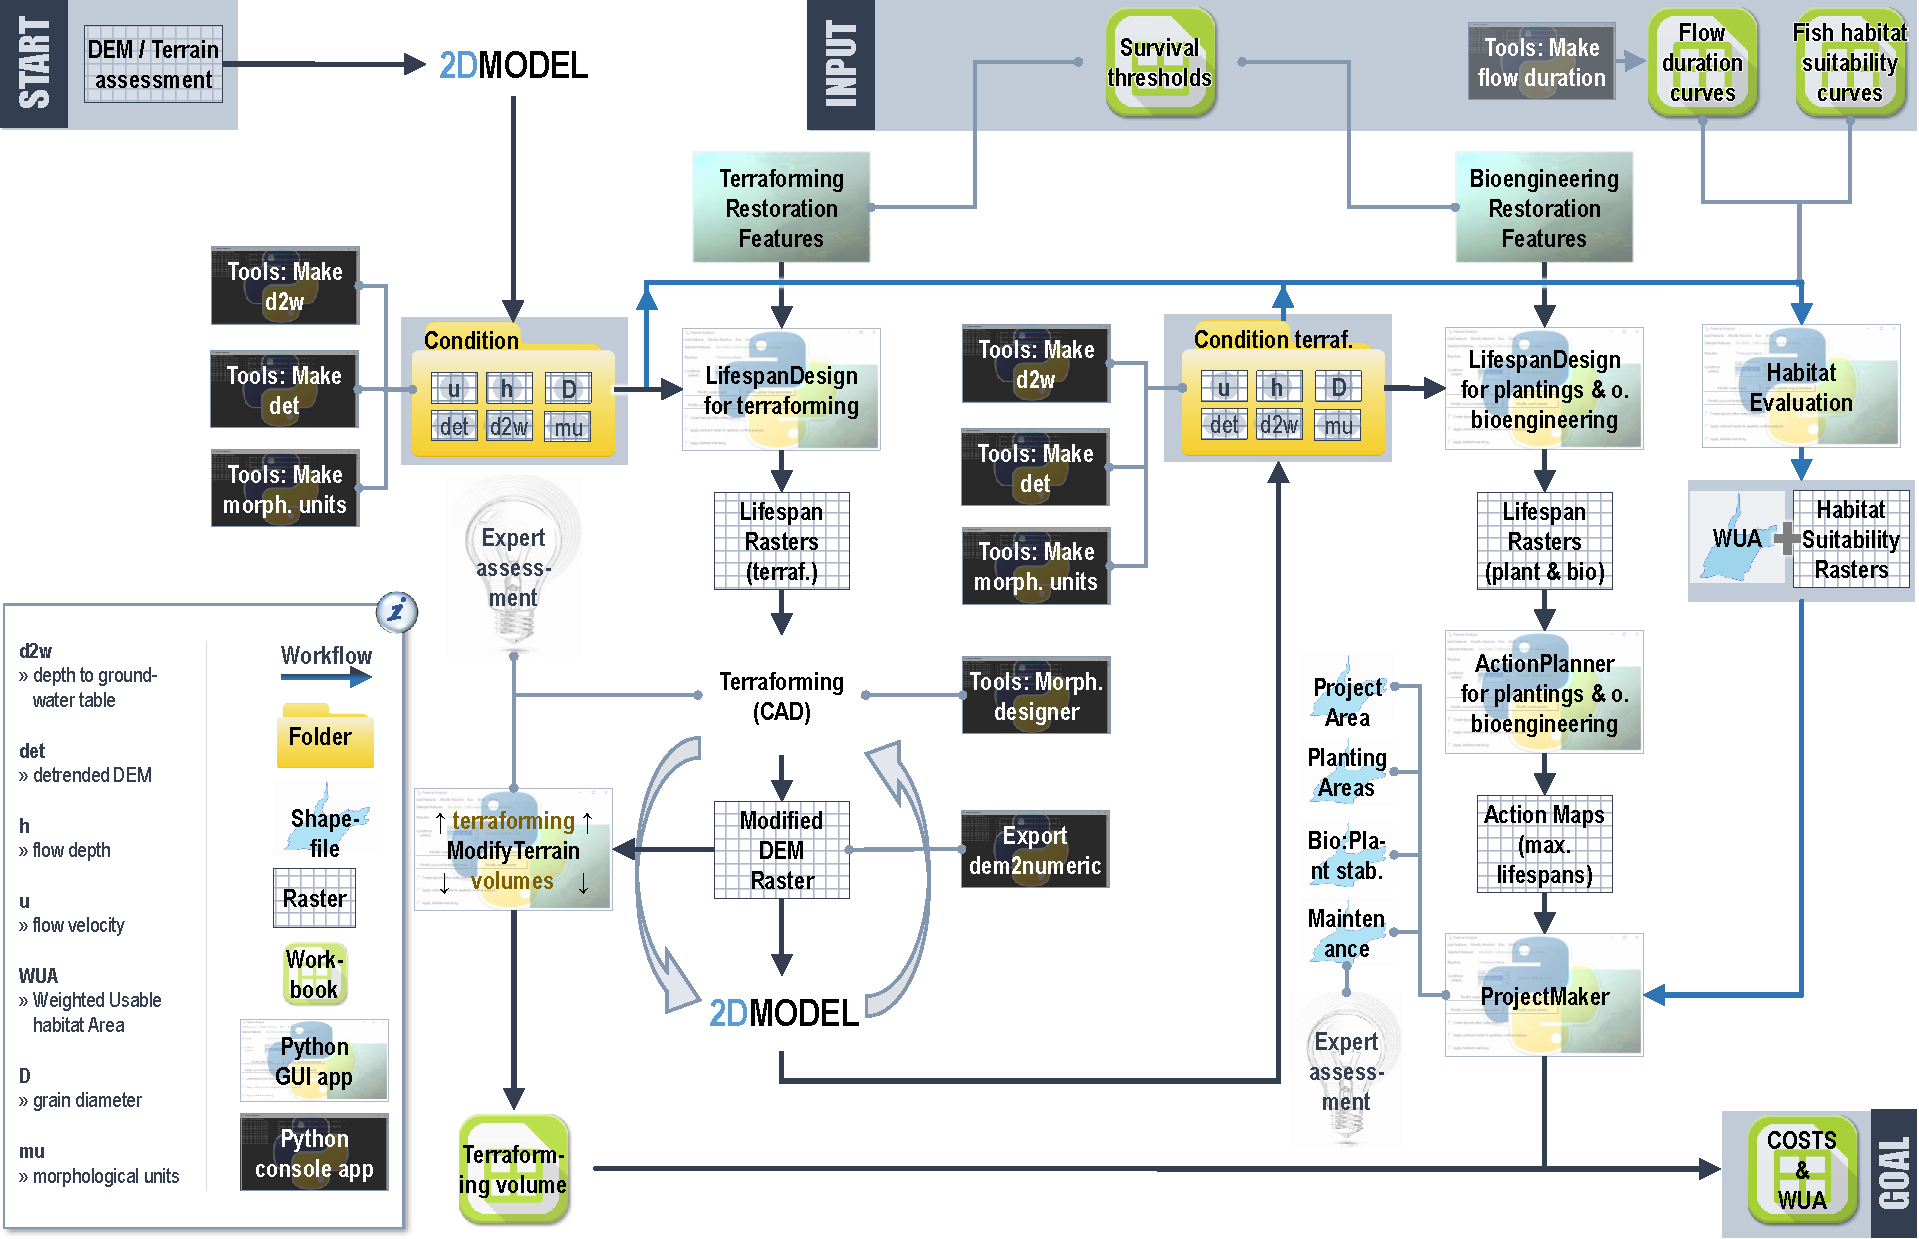
\includegraphics[width=1.0\columnwidth]{flowchart.pdf} % Example image
	\caption{Flowchart for designing habitat enhancing stream restoration projects with the \textit{River Architect}'s modules.\label{fig:flowchart}}
	\end{center}
\end{figure}

The procedure of project design following the flowchart involves the following steps:
\begin{enumerate}
	\item Generate a terrain elevation model (DEM).
	\item Determine relevant discharges for 2D hydrodynamic modeling:
	\begin{itemize}
	  \item At least three annual discharges describing the "most of the time" - situation of the considered river for habitat evaluation assessments. \textit{River Architect}'s \textit{Tools} contain scripts for generating flow duration curves from gaging station data.
	  \item At least three flood discharges against which potential restoration features have to withstand (determine lifespan intersects).
	\end{itemize}
	\item Run a 2D hydrodynamic model (steady) with all determined discharges to generate hydraulic snap-shots of the river.
	\item Compile a raster database of existing (pre-project) river conditions, including:
	\begin{itemize}
		\item A	detrended digital elevation model (see \textit{River Architect}'s \textit{Tools});
		\item Flow depth and velocity for multiple discharges Rasters from 2D hydrodynamic modeling (see Sec.~\ref{sec:input});
		\item A substrate map (\texttt{dmean} for metric or \texttt{dmean{\myUnderscore}ft} for U.S. customary units); relevant methods are described in \citet{detert18, staehly17, jackson13}; 
		\item Datasets that can be used to assess design feature stability, such as side channel design criteria (e.g., Sec.~\ref{sec:sidechnl});
		\item Terrain change Rasters \citep[Topographic Change Detection or DEM differencing according to][]{wyrick16};
		\item A depth to groundwater table Raster (see \textit{River Architect}'s \textit{Tools});
		\item A morphological unit Raster \citep[see \textit{River Architect}'s \textit{Tools} applying methods from][]{wyrick14b}.
	\end{itemize}
	\item Apply \textit{LifespanDesign} module to framework (terraforming) features.
	\item \textit{LifespanDesign} maps and expert assessment serve for the identification of relevant terraforming features.
	\item Iterative terraforming application (if relevant):
	\begin{itemize}
	  \item Use the \textit{ModifyTerrain} module for systematic terrain grading or broaden the river bed, however, adaptations are required and computer-aided design must be manually applied to modify the existing (pre-project) DEM, where the \textit{Tools} provide assistance for designing self-sustaining pool-riffle channels.
	  \item Re-compile the flow depth an velocity maps (re-run 2D model) with the modified DEM, where the \textit{Tools} provide routines for converting between raster types.
	  \item Verify the suitability of the modified DEM (e.g., barrier height to ensure flood safety); if the verification show weaknesses, adapt the terraforming and re-compile the flow depth and velocity maps until terraforming is satisfactory.
	  \item Use the \textit{ModifyTerrain} module for comparing pre- and post project DEMs to determine required excavation and fill volumes.
	\end{itemize}	
	\item Apply the \textit{LifespanDesign} module to vegetation plantings and (other) bioengineering features based on the terraformed DEM (or the original DEM if no terraforming applies).
	\item Use the \textit{MaxLifespan} module to identify best performing (highest lifespan) vegetation plantings and bioengineering features.
	\item If the soils are too coarse, apply the maintenance feature of "incorporate fine sediment in soils" to ensure that planned vegetation plantings can grow.
	\item If gravel augmentation methods are applicable: Consecutively apply the \textit{LifespanDesign} and \textit{MaxLifespan} module to maintenance features to foster self-sustaining, artificially created morphological patterns within the terraforming process.\\
	If gravel is added in-stream, re-run the numerical model for the assessment of gravel stability with the \textit{LifespanDesign} module and the combined habitat suitability with the \textit{HabitatEvaluation} module to compare the Annually Usable habitat Area before and after stream restoration.
	\item Use the \textit{HabitatEvaluation} to assess the "existing" (pre-project) and "with implementation" (post-project) habitat suitability in terms of annually usable habitat area (AUA).
	\item Use the \textit{ProjectMaker} to calculate costs, net gain in AUA, and their ratio as a metric defining the project trade-off.
\end{enumerate}

The working principles of the \textit{LifespanDesign}, \textit{MaxLifespan}, \textit{ModifyTerrain}, \textit{HabitatEvaluation}, and \textit{ProjectMaker} modules are explained in chapters \ref{part:lf}, \ref{part:ap}, \ref{part:mt}, \ref{part:he}, and \ref{part:pm}, respectively. The differentiation between terraforming (framework), planting and other bioengineering, and maintenance features is described in Sec.~\ref{sec:featoverview}. The correct installation of the \textit{River Architect} package and setting the good code environment is explained in the following Sec.~\ref{sec:req}.

\section{Package structure, requirements and logfiles} \label{sec:req}
\subsection{File structure}
The main directory (\texttt{/RiverArchitect/}) contains the documentation file, a \texttt{Tools} folder, and a template folder tree named \texttt{/\textit{NewRiver}/}. This template folder contains the program launcher named\\ \texttt{LAUNCH{\myUnderscore}River Architect{\myUnderscore}WINx64.bat} and the Python~2.7 file \texttt{stream{\myUnderscore}restoration{\myUnderscore}gui.py} with routines called by the launcher. The \textit{River Architect} modules are located in sub-folders of \texttt{/\textit{NewRiver}/}. Thus, the master folder (\texttt{/RiverArchitect/}) includes the following files and directories:
\begin{itemize}
	\item \textbf{.site{\myUnderscore}packages}\\
	Contains adapted third-party Python packages and own packages
	\begin{itemize}
		\item \texttt{openpyxl}\\
		Contains a modified version of the \pythoninline{openpyxl} (version 2.5.2) package for \textit{River Architect}
		\item \texttt{riverpy}\\
		Package-own python scripts with recurring routines and classes that are used in multiple modules.
		\begin{itemize}		
			\item \texttt{cDefinitions.py} contains inter-module information of reach and feature keywords.
			\item \texttt{cGravel.py} contains subfeatures of the Gravel augmentation-feature in \texttt{cFeatures}.
			\item \texttt{cPlants.py} contains subfeatures of the Plantings-feature in \texttt{cFeatures} and the \texttt{ModifyTerrain} module.
			\item \texttt{cTerrainIO.py} applies on the \pythoninline{openpyxl} package the assessment of reach information and for writing calculated volumes to xlsx output.
			\item \texttt{fGlobal.py} provides functions that are required in this module and the other modules in several classes.
		\end{itemize}
	\end{itemize}
	\item \textbf{00{\myUnderscore}Documentation}\\
	Contains this manual.
	\item \textbf{\textit{NewRiver}/01{\myUnderscore}Conditions}\\
	This folder contains \texttt{\textit{condition}} folders with parameter Rasters. The condition name begins with a 4-digit year number (e.g., \texttt{2008}), optionally followed by a 3-characters reach ID (e.g., \texttt{xyz}) and a feature layer indicator (e.g., \texttt{lyr01} for terraforming features). The syllables are separated by an underscore. The process of defining of reaches is explained in Sec.~\ref{sec:introsetreaches} and Sec.~\ref{sec:mtsetreaches}. The setting of feature layers is introduced in Sec.~\ref{sec:modfeat}.
	\item \textbf{Module (folder): \texttt{\textit{NewRiver}/LifespanDesign}}\\
	Lifespan and Design analyses of restoration features (see Manual Chapter~\ref{part:lf}).
	\begin{itemize}
		\item \texttt{Output} folder with sub-folders for \texttt{Mapping} and \texttt{Rasters} from individual module runs.
		\item \texttt{Products} folder with sub-folders \texttt{Layouts}, \texttt{Maps} and \texttt{Rasters} for manually storing results from relevant module runs.
		\item \texttt{.cache} folder occurs temporarily when the module is executed.
		\item \texttt{.templates} folder should not be modified and contains input (\texttt{*.inp}) files; if required, the module includes routines for changing the input files.
		\item \texttt{cFeatureLifespan.py} contains stream restoration features classes with pointers to parameters and threshold values.
		\item \texttt{cLifespanDesignAnalysis.py} contains GIS-based functional core for processing \texttt{Raster} files.
		\item \texttt{cMapLifespanDesign.py} contains routines creating layout files (\texttt{mxd}) and \texttt{PDF} maps.
		\item \texttt{cParameters.py} contains the parameter input core with pointers to \texttt{Raster}s and \texttt{Raster} names.
		\item \texttt{cReadInpLifespan.py} contains classes that read input data from \texttt{*.inp} files.
		\item \texttt{cThresholdDirector.py} provides the ThresholdDirector class for reading threshold values from spreadsheet ``thresholds''.
		\item \texttt{feature{\myUnderscore}analysis.py} coordinates class instantiations and function calls.		
		\item \texttt{lifespan{\myUnderscore}design{\myUnderscore}gui.py} is a standalone script that creates the graphical user interface (GUI) for running the \textit{LifespanDesign} module.
		\item \texttt{LAUNCH{\myUnderscore}Windows{\myUnderscore}x64.bat} is a batchfile that runs \texttt{lifespan{\myUnderscore}design{\myUnderscore}gui.py}.
	\end{itemize}
	\item \textbf{Module (folder): \texttt{\textit{NewRiver}/MaxLifespan}}\\
	Action planner in folder \texttt{MaxLifespan} (see Manual Chapter~\ref{part:ap})
	\begin{itemize}
		\item \texttt{Output} folder with sub-folders for \texttt{Layouts}, \texttt{Maps} and \texttt{Rasters} from individual module runs.
		\item \texttt{Products} folder with sub-folders \texttt{Layouts}, \texttt{Maps} and \texttt{Rasters} for manually storing results from relevant module runs.
		\item \texttt{.cache} folder occurs temporarily when the module is executed.
		\item \texttt{.templates} folder contains additional Rasters, which are required by this module; other Rasters are loaded from \textit{01{\myUnderscore}Conditions}.
		\item \texttt{action{\myUnderscore}gui.py} is a standalone script that creates the graphical user interface (GUI) for running the \textit{MaxLifespan} module.
		\item \texttt{action{\myUnderscore}planner.py} coordinates class instantiations and function calls.
		\item \texttt{cActionAssessment.py} contains the GIS-based functional core that identifies optimum lifespans and associated features by processing lifespan/design \texttt{Raster} and \texttt{shape} files.
		\item \texttt{cFeatureActions.py} contains pointers to stream restoration feature data in the \textit{LifespanDesign} module.
		\item \texttt{cMapActions.py} coordinates layout and action map creation.
		\item \texttt{cReadActionInput.py} contains functions for reading \texttt{*.inp} files from the \texttt{.templates} folder.
		\item \texttt{LAUNCH{\myUnderscore}Windows{\myUnderscore}x64.bat} is a batchfile that runs \texttt{action{\myUnderscore}planner{\myUnderscore}gui.py}.
	\end{itemize}
	\item \textbf{Module (folder): \texttt{\textit{NewRiver}/ModifyTerrain}}\\
	Performs half-automated terrain modifications and calculates excavation / fill volumes of terraforming features (see Manual Chapter~\ref{part:mt}).
	\begin{itemize}
		\item \texttt{Input} folder containing optional modified DEMs for volume difference assessment.
		\item \texttt{Output} folder with sub-folders \texttt{Logfiles} and \texttt{Rasters} from individual module runs.
		\item \texttt{Products} folder with sub-folders \texttt{Logfiles} and \texttt{Rasters} for manually storing results from relevant module runs.
		\item \texttt{.cache} folder occurs when the module is executed.
		\item \texttt{.templates} folder contains additional Rasters, which are required by this module; other Rasters are loaded from \texttt{01{\myUnderscore}Conditions}.		
		\item \texttt{cMapModifyTerrain.py} provides routines for the layout creation and mapping of modified DEMs and volume/terrain elevation differences.
		\item \texttt{cModifyTerrain.py} contains GIS-based functional core for modifying DEM \texttt{Raster} files and calculating volumes using ArcGIS ``3D'' extension.		
		\item \texttt{modify{\myUnderscore}terrain{\myUnderscore}gui.py} is a standalone script that creates the graphical user interface (GUI) for running the \textit{ModifyTerrain} module
		\item \texttt{LAUNCH{\myUnderscore}Windows{\myUnderscore}x64.bat} is a batchfile that runs \texttt{modify{\myUnderscore}terrain{\myUnderscore}gui.py} on Windows x64.
	\end{itemize}
	\item \textbf{Module (folder): \texttt{\textit{NewRiver}/HabitatEvaluation}}\\
	Creates Habitat Suitability Index Rasters / maps and quantifies annually usable habitat area for target fish species and a user-defined range of discharges (see Manual Chapter~\ref{part:he}).
	\begin{itemize}
		\item \texttt{CHSI} contains subfolders with with composite habitat suitability index Rasters for pre- and post-project \texttt{conditions}.
		\item \texttt{FlowDurationCurves} contains workbooks with flow duration curves (exceedance probabilities). Refer to the external \texttt{Tools} to generate appropriate \texttt{Spreadsheets}.
		\item \texttt{HSI} contains subfolders with with habitat suitability index \texttt{Rasters} for pre- and post-project \texttt{conditions}.
		\item \texttt{AUA} contains result workbooks with AUA values for examined \texttt{conditions}. The \texttt{Rasters} subfolder contains the associated composite habitat suitability Rasters.
		\item \texttt{.cache} folder occurs temporarily when the module is executed.
		\item \texttt{.templates} folder contains spreadsheet templates for the quantification of annually usable habitat area and the definition of fish species, lifestages and associated habitat suitability curves.
		\item \texttt{cFish.py} contains the \pythoninline{Fish} class that reads characteristic species and lifestage data from \texttt{.templates/Fish.xlsx}.
		\item \texttt{cHabitatIO.py} uses the \pythoninline{openpyxl} package to read and write data from and to \texttt{xlsx} files, respectively.
		\item \texttt{cHSI.py} contains the \pythoninline{CHSI}, \pythoninline{HHSI} and \pythoninline{FlowAssessment} classes to calculate composite habitat suitability Rasters, hydraulic habitat suitability Rasters and interpolating the annual flow duration of considered discharges.
		\item \texttt{habitat{\myUnderscore}gui.py} contains the \pythoninline{MainGui} class of this module.
		\item \texttt{sub{\myUnderscore}gui{\myUnderscore}hhsi.py} opens a new GUI window to create hydraulic habitat suitability Rasters and determine associated annual flow duration.
		\item \texttt{LAUNCH{\myUnderscore}Windows{\myUnderscore}x64.bat} is a batchfile that runs \texttt{habitat{\myUnderscore}gui.py} on Windows x64.
	\end{itemize}
	\item \textbf{Module (folder): \texttt{\textit{NewRiver}/ProjectMaker}}\\
	Applies on results from \textit{MaxLifespan} and \textit{HabitatEvaluation}, as well as manual inputs to calculate project cost-benefit metrics (see Manual Chapter~\ref{part:pm}).
	\begin{itemize}
		\item \texttt{.cache} folder occurs temporarily when the module is executed.
		\item \texttt{.templates} folder contains a template folder tree and template workbooks with unit cost tables, as well as sample application data that illustrate potential results of the module.
		\item \texttt{cIO.py} uses the \pythoninline{openpyxl} package to read and write data from and to \texttt{xlsx} files, respectively.
		\item \texttt{cWUA.py} applies on \textit{HabitatEvaluation} results, in particular CHSI Rasters for calculating AUA in the project area.
		\item \texttt{fFunctions.py} contains module-specific functions.
		\item \texttt{project{\myUnderscore}maker{\myUnderscore}gui.py} contains the \pythoninline{MainGui} class of this module.
		\item \texttt{s20{\myUnderscore}plantings{\myUnderscore}delineation.py} applies on \textit{MaxLifespan} products for assessing most suitable vegetation plantings within the project area.
		\item \texttt{s21{\myUnderscore}plantings{\myUnderscore}stabilization.py} applies on \textit{MaxLifespan} products and user-defined input parameters for mapping bioengineering futures required in order stabilize vulnerable vegetation plantings.
		\item \texttt{s40{\myUnderscore}compare{\myUnderscore}wua.py} applies on \textit{HabitatEvaluation} CHSI rasters used in \texttt{cWUA.py} for assessing the annually usable habitat area for a target fish species and lifestage within the project area.
		\item \texttt{LAUNCH{\myUnderscore}Windows{\myUnderscore}x64.bat} is a batchfile that runs \texttt{habitat{\myUnderscore}gui.py} on Windows x64.
	\end{itemize}
	\item \textbf{Folder: \texttt{Tools}}\\
	Applies on results from \textit{MaxLifespan} and \textit{HabitatEvaluation}, as well as manual inputs to calculate project cost-benefit metrics (see Manual Chapter~\ref{part:pm}).
	\begin{itemize}
		\item \texttt{.cache} folder occurs temporarily when the module is executed.
		\item \texttt{.templates} folder contains a template workbooks for multiple purposes.
		\item \texttt{Products} folder contains results of any script in this folder.
		\item \texttt{cDepth2Groundwater.py} provides routines for calculating depth to groundwater Rasters.
		\item \texttt{cDetrendedDEM.py} provides routines for generating detrended DEM Rasters.
		\item \texttt{cHydraulic.py} contains a \pythoninline{Hydraulic} class with routines for calculating cross-section-averaged flow characteristics.
		\item \texttt{cInputOutput.py} contains classes required for reading and writing data, as well as calculation progress logging.
		\item \texttt{cMorphUnit.py} provides routines for calculating instream morphological units \citep{wyrick14b}.
		\item \texttt{cPoolRiffle.py} provides routines for designing self-sustaining pool-riffle channels.
		\item \texttt{fTools.py} is a set of functions used by other Python applications within this folder.		
		\item \texttt{make{\myUnderscore}annual{\myUnderscore}peak.py} prepares required input data for statistic flow analyses and with the U.S. Army Corps of Engineers' \texttt{HEC-SPP} software.
		\item \texttt{make{\myUnderscore}d2w.py} calculates depth to groundwater Rasters (uses \texttt{cDepth2Groundwater.py}).
		\item \texttt{make{\myUnderscore}det.py} calculates detrended DEM Rasters (uses \texttt{cDetrendedDEM.py}).
		\item \texttt{make{\myUnderscore}flow{\myUnderscore}duration.py} creates flow duration curves (annual averages) for the assessment of AUA.
		\item \texttt{make{\myUnderscore}mu.py} calculates instream morphological unit Rasters (uses \texttt{cMorphUnit.py}).
		\item \texttt{morphology{\myUnderscore}designer.py} creates design tables for self-sustaining pool-riffle channels (uses \texttt{cHydr aulic.py} and \texttt{cPoolRiffle.py}).
		\item \texttt{run{\myUnderscore}make{\myUnderscore}\ldots{}.bat} are a batchfiles that run \texttt{make{\myUnderscore}\ldots{}.py} on Windows x64.
		\item \texttt{run{\myUnderscore}morphology{\myUnderscore}designer.bat} are a batchfiles that run \texttt{morphology{\myUnderscore}designer.py} on Windows x64.
	\end{itemize}
\end{itemize}

\subsection{Additional River Architect Tools} \label{sec:tools}
Beyond the fully automated generation of many Raster and shapefile types for stream restoration, an additional Toolbox is available that helps to prepare input files such as detrended digital elevation models, depth to groundwater Rasters or flow duration curves. Moreover, routines for the hydraulic design of pool-riffle sequences or flood analysis are available, where the flood analysis applies on the U.S. Army Corps of Engineers' \texttt{HEC-SPP} software. The \textit{Tools} routines are located in \texttt{RiverArchitect/Tools/}. Using the tool routines (\textit{Python} files) requires basic knowledge of \textit{Python} and manual modifications of particular codes.

\subsection{Requirements}
The execution of \textit{River Architect} requires the following external packages to be installed, which are part of the standard ArcGIS -- \texttt{python} installation: \pythoninline{arcpy}, \pythoninline{arcpy.sa}, \pythoninline{argparse}, \pythoninline{glob}, \pythoninline{logging}, \pythoninline{os}, \pythoninline{shutil}, \pythoninline{subprocess} (not mandatory, also works without this package), \pythoninline{sys}, \pythoninline{Tkinter}, and \pythoninline{__future__}. Furthermore, the \textit{River Architect} package requires ArcGIS' ``Spatial Analyst'' and ``3D'' (ModifyTerrain only) extensions.\\
The call of the GUIs from the individual module batch files (\texttt{LAUNCH{\myUnderscore}Windows{\myUnderscore}x64.bat}) is designed for Windows (x64) but can be easily changed to UNIX operating systems given that ArcGIS is installed. However, the \textit{River Architect} package was currently only tested on Windows platforms.\\
Any folder beginning with a ``.'' as for example \texttt{.cache}, \texttt{.idea} or \texttt{.ReferenceLayouts} must not be modified or assessed by any other program, in particular during the execution of package methods. Files stored in \texttt{.templates} folders are directly called by the GUIs if user definitions are admitted.\\
At the end of an execution, the applied modules have created their output folders, which are indicated in the command prompt.\\
A spreadsheet editing software such as \textit{Excel} or \textit{OpenOffice} is required for modifications of user definitions.


\subsection{Logfiles}
Logfiles \texttt{.log} are created in the module directories during every run task. These files contain time-stamped terminal messages of program activities, warnings and error messages. Thus, logfiles enable the user to review process duration and to trace back problems. The handling of potential errors and warning messages are listed in Chapter~\ref{part:troub} with descriptions of problem sources and solutions.

\section{Getting started (GUI)}\label{sec:gui}

\subsection{Prepare file structure}\label{sec:prepdir}
The first step is to copy the template file structure (\texttt{NewRiver} folder) in \textit{River Architect} and to rename the copy corresponding to the name of the analyzed river.

\subsection{Program environment setup and batchfile modification}
The package is designed for an ArcGIS Python \textbf{x64} interpreter (ArcGIS 10.5 or higher -- older versions use the standard ArcGIS \texttt{python.exe}). The appropriate Windows (x64) \texttt{python} interpreter is typically stored in \texttt{"C:{\textbackslash}Python27{\textbackslash} ArcGISx64XX.X{\textbackslash}python.exe"}. Please note the importance of using the \textbf{x64} version: The 32-bit version will result in \texttt{ERROR 999998: Unexpected Error}.\\

Before launching the \textit{River Architect} package for the first time, the batch files need to be adapted to the system environment. On Windows, set the batch file environment as follows:

\begin{enumerate}
	\item Right-click on \texttt{LAUNCH{\myUnderscore}River Architect{\myUnderscore}WIN64.bat} and choose \textit{Edit with \textit{Texteditor}} or \textit{Open with ...} and choose a \textit{Texteditor} software.
	\item Check, and if necessary, replace the path to the good python interpreter:\\
	\textit{Default:} \texttt{"C:{\textbackslash}Python27{\textbackslash}ArcGISx64XX.X{\textbackslash}python.exe"}
	\item The string \texttt{$\%$cd$\%$} automatically points to the folder where the GUI is located.
	\item Save \texttt{LAUNCH{\myUnderscore}River Architect{\myUnderscore}WINx64.bat} and close \textit{Texteditor}.
	\item Set default application to open input file type documents (\texttt{*.inp} files):\\
	\textit{Go to folder \texttt{...{\textbackslash}River Architect{\textbackslash}LifespanDesign{\textbackslash}.templates{\textbackslash}} and right-click on \texttt{mapping.inp} to access the menu \texttt{Open with ...}. Choose any text editor, such as \texttt{Notepad}, \texttt{Texteditor} or \texttt{Notepad++} and click \texttt{OK}}.
\end{enumerate}

Apply the procedure repetitively to the \texttt{LAUNCH{\myUnderscore}Windows{\myUnderscore}x64.bat} stored in the modules sub-folders for setting individual launches. Adapt the directories of the GUI creator according to the corresponding module GUI maker ending on \texttt{...{\myUnderscore}gui.py}.\\
On UNIX platforms (Apple or Linux), make sure that the python interpreter is version 2.7 and that it can import the \pythoninline{arcpy} package. Then, open the system terminal, navigate to the directory where the package is installed (location of \texttt{.py} files) and type: \texttt{./LAUNCH{\myUnderscore}UNIX.sh}.\\

After editing the batch files, launch \textit{River Architect} by double-clicking on\\ \texttt{LAUNCH{\myUnderscore}River Architect{\myUnderscore}WINx64.bat}.

\subsection{Welcome GUI}
The \textit{River Architect} package starts in a GUI now (Fig.~\ref{fig:gui_start}), which contains three buttons to launch one of the package modules. Please note that the main window will close and a new GUI window will open. The options of the module GUIs are described in the corresponding chapters (see ``Quick GUI to ...'').\\
Alternatively, modules can be individually launched by double-clicking on \texttt{LAUNCH{\myUnderscore}Windows{\myUnderscore}x64.bat} in the corresponding module folders. Moreover, the lifespan and design map module can be executed as a standalone python script, which is described in the module chapter~\ref{part:lf}.

\begin{figure}[!hbt]
	\begin{center}
	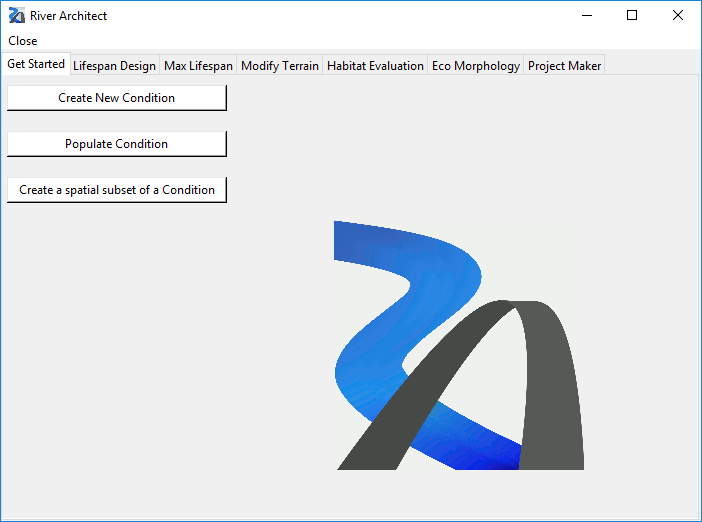
\includegraphics[width=0.4\columnwidth]{gui_start.PNG} % Example image
	\caption{\texttt{River Architect} GUI start up window. \label{fig:gui_start}}
	\end{center}
\end{figure}

\section{Restoration features}\label{sec:featoverview}
The \textit{River Architect} package differentiates between feature layers that actively modify the terrain (terraforming features), vegetation plantings features as well as (soil-) bioengineering features that provide direct aid for habitat enhancement or stabilize terrain modifications, and features that maintain artificially created, habitat enhancing morphological units (maintenance features). The features can be modified in the \textit{LifespanDesign} module's thresholds workbook (\texttt{.../RiverArchitect/LifespanDesign/.templates/threshold{\myUnderscore}values.xlsx}), which can be open from the GUI's whenever needed. Changes in this workbook should limit to cells with \texttt{INPUT}-type formatting and only \texttt{Feature Names} and \texttt{FeatureID}s of vegetation plantings should be modified. Other modifications may cause calculation instabilities or program crashes. The following list provides an overview on default features, where \textit{shortname}s occur in output file names of Rasters, layouts, PDF-maps, and spreadsheets and plantings 

\begin{itemize}
	\item \textbf{Terraforming features} modify the terrain elevation:
	\begin{itemize}
		\item Backwater, representative for swale and slackwater creation (\textit{shortname: backwt})
		\item Berm Setback (Widening, \textit{shortname: widen})
		\item Grading of terrain (Bar and Floodplain Lowering \textit{shortname: grade})
		\item Side Cavities (Bank Scalloping or Groins, \textit{shortname: sideca})
		\item Side Channels, representative for Anabranches, Multithread- or Anastomosed Channels and Flood Runners (\textit{shortname: sidech})
	\end{itemize}
	\item \textbf{Plantings features} are up to four vegetation plantings that can be defined in the \textit{LifespanDesign} module's \texttt{threshold{\myUnderscore}values.xlsx} workbook. The default plant species are (can be modified, except for the fields that are marked for input in the thresholds workbook):
	\begin{itemize}
		\item (Fremont) Cottonwood (\textit{Populus Fremontii}, \textit{shortname: cot})
		\item Box Elder (\textit{Acer Negundo}, \textit{shortname: box})
		\item White Alder (\textit{Alnus Rhombifolia}, \textit{shortname: whi})
		\item Willows (\textit{Salix Goodingii / various}, \textit{shortname: wil})
	\end{itemize}
	\item \textbf{Toolbox features} have a direct effect on habitat suitability and stabilize terrain modifications (framework features). The features are considered:
	\begin{itemize}
		\item Engineered Log Jams and instream wood placement including rootstocks (\textit{shortname: elj})
		\item Angular boulders (rocks), representative for bolder or rock placements (\textit{shortname: rocks})
		\item Other soil-bioengineering for terrain (slope) stabilization comprise for instance brush layers and / or fascines
	\end{itemize}
	\item \textbf{Complementary features} enhance the stability of artificial river systems that result from framework and toolbox features, such as:
	\begin{itemize}
		\item Sediment Replenishment (instream, \textit{shortname: gravin})
		\item Stockpiles of gravel or Gravel Augmentation (on banks or floodplain, \textit{shortname: gravou})
		\item Incorporation of Fine Sediment in soils to increase the survivorship of plantings (\textit{shortname: fines})		
	\end{itemize}
\end{itemize}

In addition, the package provides the option of limiting restoration feature maps to zones of low habitat suitability (see details in the descriptions of the \textit{HabitatEvaluation} module, part \ref{part:he}).

\section{Conditions, input Rasters and folder management} \label{sec:input}

A \textit{condition} folder filled with Rasters corresponding to the analyzed situation needs to be prepared in \texttt{RiverArchitect /01{\myUnderscore}Conditions/} folder. For example, if feature lifespans need to be assessed based on the situation in the year 2008, the condition folder name is \texttt{2008} and the Raster input folder is \texttt{/01{\myUnderscore}Conditions/2008/}. The \texttt{\textit{condition}} name may NOT include any SPACE character and the initial condition should correspond to a 4-digit year.\\
The five modules provide options to process input data according to the defined starting condition year. The modules create output folders beginning with the 4-digit year and automatically append feature layer (cf. Sec.~\ref{sec:modfeat}) and reach (cf. Sec.~\ref{sec:mtsetreaches}) information.\\

The input Rasters need to be in (ArcGIS) GRID format, notably, a \texttt{\textit{Raster{\myUnderscore}name}.aux.xml} file and an \texttt{\textit{Raster{\myUnderscore}na me}} folder with \textit{adf} and \textit{xml} files.
Depth Raster names must start with \texttt{h} and velocity Raster names must start with \texttt{u}, followed by a three digit discharge \texttt{QQQ}, which is independent of the unit system. If the discharge is larger than 1000~cfs (or 1000~m$^3$/s), the letter \texttt{k} must be appended. For example, a flow depth Raster associated with a discharge of 55~cfs needs to be called \texttt{h055} and a velocity Raster associated with a discharge of 11000~cfs needs to be called \texttt{u011k}. Likewise, a flow depth Raster associated with a discharge of 55~m$^3$/s needs to be called \texttt{h055}. Thus, the Raster names ignore discharge digits after the decimal point for discharges smaller than 1000~cfs or m$^3$/s and three digits to the left of the decimal point for discharges larger than 1000~cfs or m$^3$/s. Moreover, every flow depth Raster requires a matching velocity Raster and vice verse; e.g., \texttt{h055} requires a Raster called \texttt{u055}.\\

The \pythoninline{arcpy} package does not consider pixels with \texttt{noData} values and the \textit{River Architect} package has its own routines to handle \texttt{noData} during the calculation. To ensure computation stability and pertinence, the hydraulic input Rasters (flow depth and flow velocity) need to be fitted manually to set assign zero values to \texttt{noData} pixels, even in the absence of water. This can be achieved with the following formula either in python using the \texttt{arcpy.sa} package or in \textit{ArcGIS} Desktop using the \texttt{Raster Calculator} (for discharges larger than 1000~cfs or m$^3$/s): \pythoninline{Con((IsNull("hXXXk") == 1), (IsNull("hXXXk") * 0), Float("hXXXk"))} for flow depth and \pythoninline{Con((IsNull("uXXXk") == 1), (IsNull("uXXXk") * 0), Float("uXXXk"))} for flow velocity. The \texttt{XXX} values indicate that the formulae need to be applied to all \texttt{h} and \texttt{u} Rasters.\\

Relevant Raster names for calculation are defined in an input file (\texttt{.inp}) of the \textit{LifespanDesign} module (see Sec.~\ref{sec:inpfile} for details and definitions). More Rasters indicating morphological units \citep[e.g.][]{wyrick14b} or topographic change \citep[e.g.][]{carley12} as well as a detrended digital elevation model (DEM), surface grain size estimate and a depth to groundwater Raster are (optionally) required. The input preparation \textit{Tools} \texttt{make{\myUnderscore}d2w.py}, \texttt{make{\myUnderscore}det.py} and \texttt{make{\myUnderscore}mu.py} can be used to generate depth to groundwater, detrended DEM and morpholoical units Rasters, respectively.\\
A base case is provided with the \textit{River Architect} installation files. The input files of the base case (defined in the \textit{.inp} file) represent a patch of the lower Yuba River in 2008. The base case includes a set of Rasters for flood scenarios corresponding to flood return periods of $< $1.0~year, 1.2~years, 2.5~years, 4.7~years and 12.7~years, as well as a couple of annual discharges for habitat assessments. The below listed Rasters are available in \texttt{01{\myUnderscore}Conditions/2008/} for the base case \texttt{\textit{condition}}~=~\texttt{2008}. \pythoninline{Formatted font} indicates optional Rasters, which are however recommended to use because they significantly increase the pertinence of lifespan maps; Rasters written in \texttt{Courier New} font are mandatory. The Raster names correspond to the above-described naming conventions.\\
\begin{tabular}{l p{0.13\textwidth} L{0.295\textwidth} l l p{0.14\textwidth} L{0.26\textwidth}}
		\multicolumn{7}{l}{}\\ % add vspace using an empty row
		\multicolumn{3}{l}{\textbf{Flow velocity (in fps):}} & &\multicolumn{3}{l}{\textbf{Flow depth (in ft):}}\\ 
		- & \texttt{u530} & for habitat evaluation & &- & \texttt{h530} & for habitat evaluation\\
		- & \texttt{u700} & for habitat evaluation & &- & \texttt{h700} & for habitat evaluation\\
		- & \texttt{u880} & for habitat evaluation & &- & \texttt{h880} & for habitat evaluation\\
		- & \texttt{u001k} & for habitat evaluation and min. floods  & &- & \texttt{h001k} & for habitat evaluation and min. floods\\
		- & \texttt{u005k} & 1.2-years flood velocities & &- & \texttt{h005k} & 1.2-years flood depths\\
		- & \texttt{u021k} & 2.5-years flood velocities & &- & \texttt{h021k} & 2.5-years flood depths\\
		- & \texttt{u042k} & 4.7-years flood velocities & &- & \texttt{h042k} & 4.7-years flood depths\\
		- & \texttt{u084k} & 12.7-years flood velocities & &- & \texttt{h084k} & 12.7-years flood depths\\
		\multicolumn{7}{l}{}\\
		\multicolumn{3}{l}{\textbf{Topographic change (in ft):}} & &\multicolumn{3}{l}{\textbf{Depth two water table (in ft):}}\\ 
		- & \pythoninline{dodfill} & 2006/2008--2014 deposition heights & &- & \pythoninline{d2w} & referring to base flows of \\ 
		- & \pythoninline{dodscour} & 2006/2008--2014 scour depths & & & & 530--880~cfs\\
		\multicolumn{7}{l}{}\\
		\multicolumn{3}{l}{\textbf{ Morphological Units (string):}} & &\multicolumn{3}{l}{\textbf{D$_{mean}$ valley (in ft):}}\\ 
		- & \texttt{mu} & generated with \texttt{make{\myUnderscore}mu.py}  & &- & \texttt{dmean{\myUnderscore}ft} & mean valley grain size \\
		\multicolumn{7}{l}{}\\
		\multicolumn{3}{l}{\textbf{ DEM (in ft a.s.l.):}} & &\multicolumn{3}{l}{\textbf{ DEM detrended (in ft):}}\\ 
		- & \texttt{dem} & Digital Elevation Model & &- &\texttt{dem{\myUnderscore}detrend} & \texttt{make{\myUnderscore}det.py} \\
%		\multicolumn{7}{l}{}\\
%		\multicolumn{3}{l}{\textbf{ Habitat suitability (cHSI):}} & &\multicolumn{3}{l}{\textbf{Background image}}\\ 
%		- & \pythoninline{max_chsi} & Major fish species habitat suitability (COVER) & &- & \texttt{back} & Black $\&$ White image of the site from 2009\\
		\multicolumn{7}{l}{}\\
		\multicolumn{3}{l}{\textbf{Side channel}} & &\multicolumn{3}{l}{\textbf{Wildcard}}\\ 
		- & \pythoninline{sidech} & Side channel delineation  & &- & \pythoninline{wild} & 0/nodata (= off) and 1 (= on) values for any purpose to confine analysis\\
		\multicolumn{7}{l}{}\\ % add vspace using an empty row
\end{tabular}

Some parameters, such as the dimensionless bed shear stress or the mobile grain size, can be directly computed from the flow velocity, depth, and present grain size. Additional input Rasters could be used for every parameter to shorten calculation duration, but this approach required large storage capacity on the hard disk and it is less flexible regarding computation methods. Therefore, the \textit{River Architect} uses its own routines for calculating parameters such as the dimensionless bed shear stress or mobile grain sizes.

\section{Define Reaches and Features} \label{sec:define}
\subsection{Set Reaches} \label{sec:introsetreaches}
Particular rivers or reaches for the analysis can be defined from the \textit{LifespanDesign} and \textit{ModifyTerrain} GUIs, referring to:\\
\texttt{ModifyTerrain/.templates/computation{\myUnderscore}extents.xlsx}\\

The \textit{ModifyTerrain} and \textit{LifespanDesign} modules provide options for reach differentiation and limit calculations to defined particular reaches. These limitations are automatically used by the other modules. This subdivision of the computation domain enables the analysis of up to eight reaches per copy of \textit{River Architect}. Fig.~\ref{fig:illu_reaches} illustrates the \pythoninline{Reach Menu} of the \textit{ModifyTerrain} GUI. Changes can be effected by clicking on the \texttt{Reaches} dropdown menu and then \texttt{DEFINE REACHES}, or directly in the folder \texttt{ModifyTerrain/.templates/}. Detailed instructions are provided in Sec.~\ref{sec:mtsetreaches}.

\begin{figure}[hbt]
	\begin{center}
	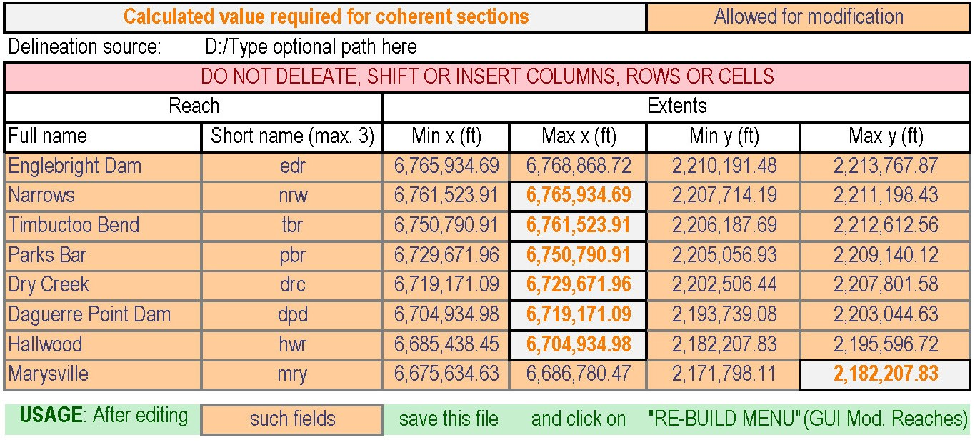
\includegraphics[width=0.75\columnwidth]{computation_extents_illu.pdf} % Example image
	\caption{Spreadsheet with reach definitions (stored in \texttt{ModifyTerrain/.templates/computation{\myUnderscore}extents.xlsx}). \label{fig:illu_reaches}}
	\end{center}
\end{figure}

If the workbook is accidentally deleted or irreparable, incorrect modifications were made, there is a backup copy available:\\
\texttt{ModifyTerrain/.templates/computation{\myUnderscore}extents - Copy.xlsx}

\subsection{Define or modify features} \label{sec:modfeat}
The \textit{LifespanDesign} module uses a spreadsheet to read threshold value for feature failures (cf. Sec.~\ref{sec:modfeat}). This spreadsheet additionally defines feature names and features IDs, which can be modified if needed. The spreadsheet can be accessed either by clicking on the \textit{LifespanDesign} GUI's The ``Modify survival threshold values'' button or directly from:\\
\texttt{/RiverArchitect/LifespanDesign/.templates/threshold{\myUnderscore}values.xlsx}\\

Modifications of feature IDs and names require careful consideration because the packages apply analysis routines as a function of the features \textit{Python} classes. Changing feature names and parameters and IDs only provides the possibility of renaming features and modifying threshold values, as well as the unit system. The feature IDs are internal abbreviations, which also determine the names of output Rasters, shapefiles, and maps. Editing feature evaluations (e.g., adding an analysis routines) requires changes in the \textit{Python} code as explained in Sec.~\ref{sec:add-feat}.\\
The workbook enables changing vegetation plantings species in columns \texttt{J} to \texttt{M}. The following columns are associated with distinct feature layers (cf. definitions in Sec.~\ref{sec:featoverview}) in the workbook:
\begin{itemize}
	\item Framework features: Columns \texttt{"E"}, \texttt{"F"}, \texttt{"G"}, \texttt{"H"}, \texttt{"I"}.
	\item Plant features: Columns \texttt{"J"}, \texttt{"K"}, \texttt{"L"}, \texttt{"M"}.
	\item Other Bioengineering features: Columns \texttt{"N"}, \texttt{"O"}, \texttt{"P"}.
	\item Maintenance features: Columns \texttt{"Q"}, \texttt{"R"}, \texttt{"S"}.
\end{itemize}

Detailed instructions for the usage of \texttt{threshold{\myUnderscore}values.xlsx} is provided in Sec.~\ref{sec:modfeat} and more information on threshold values is provided in Sec.~\ref{sec:feat}. If the spreadsheet is accidentally deleted or irreparable, incorrect modifications were made, there is a backup copy available:\\
\texttt{/RiverArchitect/LifespanDesign/.templates/threshold{\myUnderscore}values - Copy.xlsx}

